% Copyright (c) 2023-2025
% This file is part of sep3cs.
%
% sep3cs is free software: you can redistribute it and/or modify
% it under the terms of the GNU General Public License as published by
% the Free Software Foundation, either version 3 of the License, or
% (at your option) any later version.
%
% sep3cs is distributed in the hope that it will be useful,
% but WITHOUT ANY WARRANTY; without even the implied warranty of
% MERCHANTABILITY or FITNESS FOR A PARTICULAR PURPOSE.  See the
% GNU General Public License for more details.
%
% You should have received a copy of the GNU General Public License
% along with sep3cs. If not, see <http://www.gnu.org/licenses/>.
%
\section{Arquitectura}

El proyecto se construirá siguiendo la arquitectura n-Layered o multicapa que, como su nombre lo indica, se enfoca en dividir el sistema en capas lógicas siendo cada una un conjunto de clases, paquetes y subsistemas que tienen funcionalidades relacionadas y se encargan de un conjunto de tareas específicas. 

Distribuir el programa en capas o niveles posibilita una distribución jerárquica de los roles y responsabilidades del mismo lo que facilita la distribución del trabajo, cada miembro del equipo de desarrollo puede trabajar en una capa específica.

Cada capa se construye sobre la inferior inmediata, la cual provee los servicios y la funcionalidad necesarios para que la capa superior pueda funcionar correctamente. Es decir, cada capa solo se comunicará con las adyacentes a ella mediante interfaces bien definidas lo que posibilita una mejor organización y modularidad del sistema así como facilitar el mantenimiento y evolución a largo plazo.

La arquitectura tiene muchas variaciones, ya sea en las capas que se utilizan o en el orden jerárquico de las mismas. Siguiendo la lógica "mantenlo simple" se usará la versión más básica compuesta por las siguientes capas:

\begin{figure}[H]
  \centering
  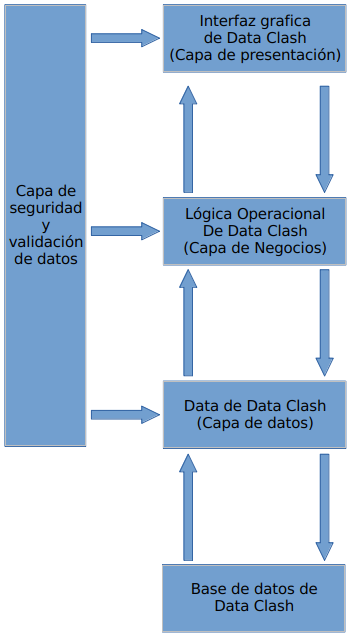
\includegraphics[width=0.36\textwidth]{../images/figure_architecture.png}
  \caption{Arquitectura por capas}
\end{figure}

\begin{enumerate}
  \item[\(\cdot\)] Capa de presentación o capa de usuario: En concreto, la interfaz gráfica, presenta el sistema al usuario, le comunica información y obtiene información o peticiones de él. Aquí es donde el usuario realizará sus peticiones de recuperación de información del juego y también donde obtendrá sus respuestas. Su requisito principal es ser lo más ‘amigable’ posible, es decir, que los conocimientos técnicos necesarios para operar esta interfaz sean mínimos de modo que esté disponible para la mayor cantidad de usuarios posibles. Esta capa se comunicará solo con la capa de negocio. 
  \item[\(\cdot\)] Capa de negocio: Aquí es donde radican los diversos programas, se reciben las peticiones del usuario a través de la capa de presentación y se computa la respuesta, enviándose nuevamente a la capa de presentación. Aquí yace el código para interpretar las solicitudes del usuario y determinar los datos que este desea recuperar, también se encarga de la actualización de los datos a través de los cambios en el juego, el primero está íntimamente relacionado con la capa de usuario mientras que el segundo es automático. También se comunica con la capa de datos para solicitar al gestor de base de datos almacenar o recuperar datos.
  \item[\(\cdot\)] Capa de datos: Es donde residen los datos y se acceden a los mismos, formada por uno o más gestores de bases de datos que realizan todo el almacenamiento de datos, reciben solicitudes de almacenamiento o recuperación de información desde la capa de negocio.
\end{enumerate}
